\documentclass{article}
\usepackage[a4paper, total={7in, 9in}]{geometry}

\usepackage{graphicx} % Required for inserting images
% \usepackage[numbers]{natbib}


\usepackage{hyperref}
\usepackage{caption}
\usepackage{multicol}
\usepackage{amsmath}
\usepackage{tabularx}
\usepackage{easyreview}
\usepackage{comment}
\usepackage{tabularx}
\usepackage{tikz}
\usetikzlibrary{trees}
\usepackage{float}
\usepackage{multirow}
%\usepackage{svg}
\hypersetup{
	colorlinks=true,
	linkcolor=black,
	urlcolor=blue,
	citecolor=blue,
	pdfborder={0 0 0},
}

\usepackage{setspace} \singlespacing
\usepackage{enumitem}
\usepackage{fontspec}
\setmainfont{FreeSerif}
\setsansfont{FreeSans}
\setmonofont{FreeMono}
\usepackage{polyglossia}
\setdefaultlanguage{english} % Main language
\setotherlanguages{arabic, farsi, hindi, bengali}
\setmainfont{CMU Serif}
\newfontfamily\arabicfont[Script=Arabic]{Amiri}
\newfontfamily\hindifont[Script=Devanagari]{Lohit Devanagari}
\newfontfamily\bengalifont[Script=Bengali]{Lohit Bengali}
\newfontfamily\persianfont[Script=Arabic]{Amiri} % Persian can use the Arabic script font
\usepackage[backend=biber, style=numeric, maxnames=1, minnames=1]{biblatex}
\addbibresource{ref.bib}  % Assuming your .bib file is named references.bib

\title{Automated Essay Scoring in Arabic and Low-Resource Indic Languages: A Systematic Literature Review}
%\author{Ahmad Shafiq Zia, Swardiantara Silalahi}
\date{September 2024}

\begin{document}    
	
	\maketitle
	\section{Introduction}
	Automated Essay Scoring (AES), also known as Automated Essay Grading (AEG) or Automated Essay Evaluation, involves using specialized computer programs to assign grades to written texts in educational settings. The goal of AES mirrors traditional scoring methods, which rely on human raters trained to apply rubrics for evaluating student responses. AES aims to replicate this process by leveraging computational models.
	
	AES models are designed to evaluate both short-form responses—often referred to as Automated Short Answer Grading (ASAG)—and more complex essay-style answers. Evaluating essays presents additional challenges due to their open-ended nature, which makes it difficult to compare them against a single correct response. Moreover, features such as essay structure, coherence, and style further complicate the evaluation process, necessitating more advanced techniques.
	
	The development of effective AES models requires substantial work in Machine Learning (ML) and Natural Language Processing (NLP). These fields are essential in capturing the unique aspects of free-text answers. Most AES models rely on supervised learning, where large labeled datasets are used to train the system to recognize syntactic and semantic features relevant to the evaluation process.
	
	AES systems provide significant advantages in terms of grading efficiency, particularly in standardized testing and online learning environments. These systems can serve multiple roles: acting as independent assessors, working alongside human examiners, or even monitoring human raters for consistency. In large-scale online learning platforms, such as Massive Open Online Courses (MOOCs), AES systems drastically reduce the time and cost associated with human grading by automating the evaluation of free-text responses for millions of learners.
	
	AES systems offer significant advantages in grading large volumes of student essays, providing faster turnaround times and reducing overall costs. Additionally, they can help mitigate biases and inconsistencies that human examiners may introduce into the grading process \cite{malouff2016bias}. Research has also focused on addressing rating biases in the training datasets used to develop these models \cite{amorim2018aesbias}.
	
	However, implementing AES systems can come with substantial time and financial costs. Achieving high accuracy and reliability requires the preparation of large, high-quality datasets. Furthermore, these models may struggle to handle unique writing styles, leading to inaccuracies. Some reliability issues can also emerge when attempting to evaluate subjective elements of essays, such as the creativity of ideas and arguments, which remain difficult to quantify. Moreover, test-takers often question the transparency of these systems. If the underlying rules of an AES model are disclosed, critics argue that students might exploit these rules to achieve higher scores than they would from human examiners.
	In our collection of papers, we observed that majority of papers tend to follow a similar approach in implementing their model.
	\subsection{Working Of An AES System}
	\begin{enumerate}
		\item \textbf{Preprocessing} The raw text is transformed into a format suitable for the AES system. This process includes removing noise and normalizing the text. Unnecessary features, such as stop words, are eliminated, and techniques like lemmatization, stemming, and tokenization are applied to prepare the text for further analysis.
		
		\item \textbf{Feature Extraction} Features are extracted from the preprocessed data using one of two approaches. The first involves manually defining and extracting a set of predetermined features, which are then used to calculate a score. However, this method is often less accurate compared to models that automatically extract features. Deep learning models, which contain multiple hidden layers in their neural networks, automatically identify and use complex features to improve prediction accuracy.
		
		\item \textbf{AES Model} The model is trained using machine learning algorithms on the extracted features. These models, which may use traditional machine learning or deep learning techniques, learn the relationship between the text features and essay scores from the training dataset. Some systems also employ a hybrid approach, combining traditional methods with machine learning to enhance accuracy.
		
		\item \textbf{Scoring} The trained model is applied to a test dataset, which may consist of essays written in response to specific prompts or more general topics. The model generates scores for these essays, and the scores are often normalized or scaled to align with the scoring standards used by human examiners.
	\end{enumerate}
	After generating scores, the model is evaluated by comparing its results on the test dataset with the scores assigned by human examiners, measuring the correlation and accuracy between the two.
	\subsection{Development of AES Systems in English Language}
	The earliest development of Automated Essay Scoring (AES) began in 1966 with the Project Essay Grader (PEG) by Ellis Paige \cite{page2003peg}. PEG assigned scores based on features such as grammar, word choice, word length, and vocabulary. The model worked by extracting these textual features and using a weighted combination to predict grades. However, since the features were considered indirect indicators of writing quality, the model was susceptible to manipulation by test-takers.
	
	Subsequent developments focused on creating AES systems that could evaluate features directly contributing to writing quality. One example is the Intelligent Essay Assessor (1999) \cite{foltz1999essayassessor}, which used Latent Semantic Analysis (LSA), a statistical technique for identifying relationships between words in a given topic. This method allowed the model to assess essay quality by comparing it to a reference text of known quality, making it more resistant to cheating and plagiarism than PEG.
	
	Other notable AES models, such as E-rater Intellimetric (2006) \cite{rudner2006intellimetric} and the Bayesian Essay Test Scoring System (BETSY) \cite{rudner2002bayes}, incorporated natural language processing (NLP) techniques. More recent advancements include the use of deep learning and transformer-based models like DeBERTa \cite{susanto2023deberta}. These trends reflect the ongoing evolution of AES models and the diverse methodologies employed over time. \textcite{ramesh2022review} provide a comprehensive review of AES in the English language.
	
	Furthermore, several US states, such as Utah and Ohio, have integrated AES systems into their educational testing programs, exemplified by tools like the Utah Compose Tool and Ohio's standardized tests.
	
	\subsection{Development of AES in Foreign languages}
	Development of AES systems in other languages depends on various factors because of the popularity of that language and the unique opportunities and challenges that language might present. Each language has different set of grammatical, and morphological rules. Therefore, they have variations in syntactic and semantic aspects of language.
	Majority of languages other than English have less resources and fewer studies. This can be due to many factors, including less number of speakers compared to popular languages (like English) or are less commonly taught in education.
	To address these challenges, work is also being done to develop multilingual models, for example,  by translating text into English for scoring. The study \textcite{firoozi2024bert} is such an example. 
	\begin{figure}
		\centering
		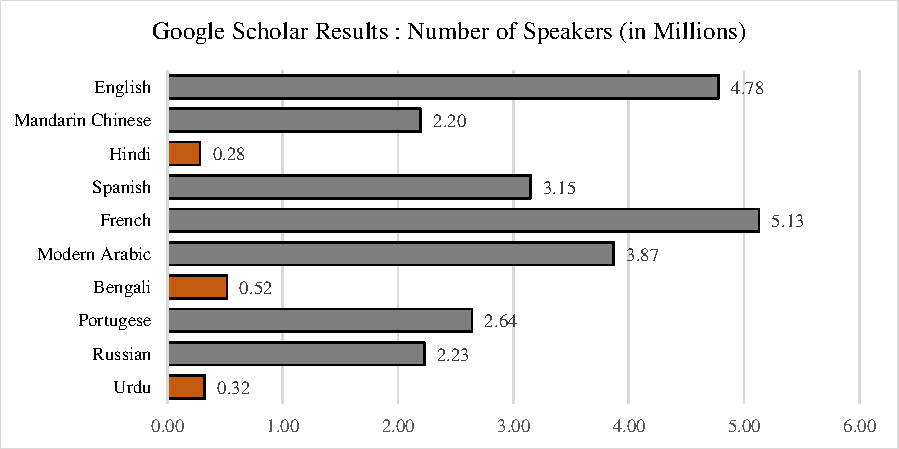
\includegraphics[width=\textwidth]{img/ratio.pdf}
		\caption{Google Scholar Results with the search query: \\
			\textit{"Automated Essay Evaluation"OR"Automated Essay Scoring" (name of language)}}
		
		\label{searchresult}
	\end{figure}
	The development of AES systems in languages other than English depends on several factors, including the popularity of the language and the unique challenges that language may present. Each language has its own set of grammatical and morphological rules, resulting in variations in syntactic and semantic structures.
	
	Most languages other than English have fewer resources and less research devoted to AES. This lack of development can be attributed to various factors, such as a smaller number of speakers compared to widely spoken languages like English or less prevalence in formal education systems. 
	
	To address these challenges, work is being done to create multilingual models, sometimes by translating text into English for scoring. \textcite{firoozi2024bert} provides an example of this approach. Different language families have distinct linguistic features that can influence how AES systems are implemented. However, the classification of language families is not universally agreed upon. As such, the discussion presented here should be regarded as a generalization, focusing primarily on well-known and widely spoken languages.
	
	Figure \ref{searchresult} shows the ratio of Google Scholar search results to the number of speakers of the top 10 most spoken languages \cite{wikitotalspeakers}. The assumption is that languages with more speakers will also have more learners, both native and non-native. While Google Scholar may not always yield relevant results, this statistic provides an estimate of AES development in these languages. The results indicate that despite having a large number of speakers, many languages—particularly those from the Indic group—have surprisingly little research. This lack of work may be due to the absence of NLP resources or insufficient datasets.
	
	Although individual languages within a family may differ in various ways, many share common features. For example, all languages in the Sino-Tibetan family (e.g., Chinese, Mandarin, Burmese) use a logographic writing system. In contrast, the Indo-European family is the largest and most diverse, containing numerous branches with distinct linguistic characteristics. While each branch has unique features, many share common root vocabulary and fundamental grammatical structures.
	
	This paper reviews the development of AES systems for widely spoken Indo-Iranian languages from the Indo-European family and Arabic from the Semitic family. These languages were selected due to their unique linguistic challenges and the author’s personal familiarity with them. The languages included in this review are:
	\begin{enumerate}
		\item Arabic
		\item Persian
		\item Hindi
		\item Bengali
	\end{enumerate}
	
	While previous literature reviews on AES systems have focused on Arabic \cite{litreviewarabic}, this paper aims to expand the scope by including recent studies on both Arabic and Indic languages. The goal is to identify trends in AES methods and explore their potential application to other low-resource languages.
	
	%\newpage
\section{Research Method}
\subsection{Research Questions}
Our review evaluates each paper based on the following research questions:
\begin{enumerate}[label=\textbf{RQ\arabic*}, leftmargin=1.5cm]
	\item What datasets are available for AES systems in the selected languages?
	\item How does each paper address preprocessing?
	\item What features and models are utilized in each paper?
	\item What are the advantages and drawbacks of the models used?
\end{enumerate}

\subsection{Search Process}
We searched well-known computer science repositories, including ACM, IEEE Xplore, Springer, ScienceDirect, and ACL, for publications from 2010 to 2024. The search strings used included terms such as “Automated Essay Scoring,” “Automated Essay Evaluation,” “Automated Essay Grading,” “AES,” and “Automated Answer Scoring,” combined with the name of the language in the search query. 

Due to the limited number of papers found, additional searches were conducted through Google Scholar and preprint platforms such as arXiv.

\subsection{Selection Criteria and Quality Assessment}
The identified papers were filtered using inclusion and exclusion criteria:
\begin{enumerate}[label=\textbf{Criteria \arabic*}, leftmargin=2cm]
	\item Only papers written in English that explicitly focus on the development and evaluation of AES systems were included.
	\item Literature review papers, thesis papers, and state-of-the-art surveys were excluded.
	\item Non-peer-reviewed papers were included only if authored by individuals affiliated with reputable institutions and with a history of peer-reviewed publications. Additionally, only papers hosted on well-established preprint servers were considered.
	\item Papers that trained models using datasets and evaluated their performance were included, while papers proposing methodologies without evaluation were excluded.
\end{enumerate}

Each selected paper was assessed for methodological rigor, considering factors such as the robustness of the research design, the reliability of the data used, and the appropriateness of the analytical techniques employed. 

Out of the 28 papers initially collected, 19 were selected based on the outlined criteria.

	\renewcommand{\arraystretch}{1.5}
	\begin{table}[]
		\centering
		\begin{tabular}{p{3in}  c}
			\hline
			\textbf{Database} & \textbf{Papers} \\ \hline
			Researchgate & 6 \\
			IEEE XPlore & 5 \\
			Sciencedirect & 2 \\
			Springer & 2 \\
			ACL & 1 \\ 
			ACM & 0 \\
			Others (Books, University Journals, Preprints) & 3 \\
			\hline
		\end{tabular}
		\caption*{Number of papers by databases}
		\label{papersbydb}
	\end{table}
	\begin{table}[]
		\centering
		\begin{tabular}{p{2in} c}
			\hline
			\textbf{Language} & \textbf{Papers} \\ \hline
			Arabic & 15 \\
			Hindi & 2 \\
			Persian & 1 \\
			Bangla & 1 \\
			\hline
		\end{tabular}
		\caption*{Number of papers by language}
		
		\label{tab:my_label}
	\end{table}
	
	
	
	\begin{comment}
		
		\subsection{Categorization of AES Systems}
		\begin{itemize}
			\item Feature based vs Neural Based Scoring \\
			Either the model is designed on basis of specific traits, or the model is trained on the basis of holistic scores. Majority of works in English utulize Kaggle's ASAP Dataset, released in 2012, for holistic scoring. Models like \cite{}
			\item Supervised and unsupervised
		\end{itemize}
	\end{comment}
\section{Linguistic Challenges}
Persian, an Indo-European language from the Iranian branch, has approximately 79 million native and non-native speakers \cite{wikitotalspeakers}. It is primarily spoken in three varieties: Standard Persian (Iran), Dari (Afghanistan), and Tajik (Tajikistan). As a pluricentric language, Persian presents challenges in NLP due to its varieties and different writing systems. While Tajik is written in a modified Cyrillic alphabet, both Dari and Standard Persian use a modified Arabic script. However, existing work has primarily focused on Standard Persian.

Persian's morphology system is largely affix-based. For instance, the word \textfarsi{بیابان} (/biyâbân/) is composed of a prefix and suffix around the root: \textit{bi} (without), \textit{âb} (water), and \textit{ân} (place suffix) — meaning desert. Moreover, these affixes can change meaning depending on the context, and in some cases, nouns can be turned into adjectives with additional affixes. Although Persian shares vocabulary with other Indo-European languages, its large influence from Arabic introduces significant loanwords.

Unlike Arabic, Persian does not have grammatical gender. Its verb construction relies on combining verb roots with prefixes, suffixes, and auxiliary verbs to express tense and meaning. The verb root is derived by removing the infinitive ending (-an). Additionally, prefixes can alter the form of the verb, while compound verbs involve both a noun or adjective.

NLP challenges in Arabic and Persian differ significantly from those in other Indo-European languages, particularly due to how short vowels are indicated. In both languages, diacritics represent short vowels but are often omitted in modern texts, adding ambiguity to the analysis. Long vowels, however, are represented with specific alphabet letters. This omission of diacritics complicates text analysis since context is necessary to derive correct meanings. For example, in Persian, \textfarsi{مرد} (/mard/) can mean \textit{man}, while \textfarsi{مِرد} (/mird/) means \textit{deceased}.

Arabic, a Semitic language, has three forms: formal (used in texts like the Quran), colloquial (for daily conversations), and Modern Standard Arabic (used formally across the Arab world). Arabic’s vowel system includes both letters (\textarabic{ا،و،ى}) and diacritics. Like Persian, modern standard and colloquial Arabic rely on context to interpret the correct meanings. For instance, the word \textarabic{ذهب} can be read as \textarabic{ذَهَبَ} (meaning ``to go") or \textarabic{ذَهَبٌ} (meaning ``gold"). Furthermore, as an agglutinative language, Arabic uses morphemes to form compound words. This, combined with words changing meaning depending on context, presents additional challenges for AES systems.

Hindi, which uses the Devanagari script, and Bengali, written in the Bengali script, are both derived from the Abugida writing system. These languages follow a consonant-vowel structure, where inherent vowels can be muted or modified with diacritics. Verb inflections modify nouns and indicate gender, number, case, politeness level, and tense. For example, in Bengali, \textbengali{তুমি} (/tumi/, meaning ``you") is informal, while \textbengali{আপনি} (/apni/) is formal. The choice of words can influence the tone and meaning of the essay. Additionally, these languages have compound words and exhibit polysemy, where words have different meanings depending on the context. For example, in Hindi, \texthindi{बाल} (/bāl/) can mean either ``hair" or ``child", making semantic analysis essential.

	\section{Resources}
	\textbf{RQ1: What are the available datasets for AES systems in the selected languages?} \\
	The papers dealt with either short, topic-specific questions or long essays. Some papers have publicly released their datasets while others have not.
	%\newpage
	%\newgeometry{bottom=1cm, top=1cm, left=1cm, right=1cm}
	\begin{table}
		\centering
		\begin{tabularx}{7in}{|c|X|p{1.5in}|p{1cm}|p{1.5cm}|}
			\hline
			Study & Dataset Size & Dataset & Type & Availability \\ \hline
			\textcite{1_gomaa2014arabic} & 610, 10 Answers for 61 questions each.  Average of 2.2 sentences and 20 words. & Egyptian Environmental Science Curriculum & Short & Private \\ \hline
			\textcite{2_shalabi2016levenshtein} & Not mentioned & Web-based, online quizzes & Short & Private \footnotemark[1] \\ \hline
			\textcite{3_shehab2018arabicsimiliarity} & 210, 21 questions, 10 students & Secondary level 3 students in a sociology course & Short & Private \\ \hline
			\textcite{4_abdeljaber2021wordnet} & 120, 30 students & Collected from a school, designed after the \href{https://www.kaggle.com/c/asap-aes}{Hewlett Foundation Dataset} & Short & Private \\ \hline
			\textcite{5_aljouie2017schoolchildren} & ~300 & Essays from grades 7-9 of intermediate schools & Long & Private \\ \hline
			\textcite{6_ghamdi2014hybridarabic} (Abbir) & 640, 200 word essay & University level Arabic course & Long & Private \\ \hline
			\textcite{7_qahtani2019rulebased} & 100, 100-250 word essays & Undergraduate and graduate students, different topics & Long & Private \\ \hline
			\textcite{8_abdel2021lcs} & 330, 33 responses for 10 questions each & School children & Short & Private \footnotemark[2] \\ \hline
			\textcite{16_rababah2017short} & Unspecified, average 4 sentences, 50 words. & Jordanian curriculum history course & Short & Private \\ \hline
			% \textcite{17_abbas2015svm}
			\textcite{18_alqahtani2020svr} & 200, essays with average length of 250 word & University level undergraduate/graduate Arabic speaking students & Long & Private \\ \hline
			\textcite{20_azmi2019aaee} (AAEE) & 350 essays & 8 topics, written by students from intermediate and secondary school students & Long & Private \\ \hline
			\textcite{22_meccawy2023mining} & ..... & Used AR-ASAG \cite{ouahrani2020ar-asag} and \textcite{16_rababah2017short} datasets & ... & ... \\ \hline
			\textcite{23_ghazawi2024bert} & 2046 essays from total of 12 questions & Undergraduate level students from various departments & Short & \href{https://osf.io/dp2nh/?view_only=4ac6373c60214ea6952855f81507fec7}{Public} \\ \hline
			\textcite{26_alsanie2022threelevels} & 293 essays & Different levels from an Arabic language learning institute & Long & Private \\ \hline
			\textcite{27_gaheen2021jaya} & 240 essays, average 79 words & Collected from ``Teaching Principles Quiz" & Short & Private \\ \hline
		\end{tabularx}
		\caption{Datasets in AES Systems for Arabic}
		\label{arabicdatasets}
	\end{table}
	%\newpage
	%\restoregeometry
	The datasets in Table \ref{arabicdatasets} are sourced from papers focused on developing AES systems. The papers dealing with short questions are labeled as "short," while those with essay-style prompts are labeled as "long." The majority of the datasets are not publicly available, although a few have their codebases accessible. Only one dataset is publicly available. 
	
	It is important to note that some papers have exclusively focused on the creation and development of corpora in Arabic. In our review, we also searched for additional datasets apart from the selected papers:
	
	\footnotetext[1]{Dataset not public, but the \href{https://github.com/albertusk95/nips-challenge-essay-scoring-arabic}{code} is available.}
	\footnotetext[2]{Only \href{https://github.com/hikmatabdeljaber/Arabic-Essay-Scoring}{codebase and a dataset sample} are public.}
	
	\begin{enumerate}
		\item \textbf{The Qatari Corpus of Argumentative Writing (QCAW) \cite{zaghouani2024qcaw} (\href{https://catalog.ldc.upenn.edu/LDC2022T04}{Public})} \\ 
		This dataset contains 390 argumentative essays, 195 of which are written in Arabic. The public dataset includes annotated parts of speech tags but lacks holistic scoring annotations.
		
		\item \textbf{QAES by \textcite{21_bashendy2024qaes} (Public)} \\ 
		This paper annotates the QCAW dataset by \textcite{zaghouani2024qcaw} by adding scores and measures including organization, vocabulary, style, etc., in addition to a holistic score. This is the only dataset with essay-style answers designed specifically for AES systems in Arabic. Although the paper claims to have the dataset publicly available, we were unable to locate it at the time of writing.
		
		\item \textbf{The Zayed Arabic English Bilingual Undergraduate Corpus (ZAEBUC) \cite{habash2022zaebuc} (\href{https://sites.google.com/view/zaebuc/home}{Public})} \\ 
		This corpus consists of 388 English and 214 Arabic annotated essays. They are collected from undergraduate freshman students in the UAE and are manually and automatically annotated for parts of speech, lemmas, and other features.
		
		\item \textbf{The Arabic Learner Corpus (ALC) (\href{https://www.arabiclearnercorpus.com/}{Private})} \\ 
		This corpus is produced using data from 942 students consisting of both native and non-native Arabic speakers and learners, with an average essay length of 178 words.
		
		\item \textbf{AR-ASAG: ARabic Dataset for Automated Short Answer Grading \cite{ouahrani2020ar-asag} (\href{https://github.com/leilaouahrani/AR-ASAG-Dataset}{Public})} \\ 
		This dataset contains 48 questions answered by 2,133 students in a cybercrimes course.
		
		\item \textbf{Arascore by \textcite{nael2022arascore} (\href{https://github.com/abdelrahmanelnaka/AraScore-Dataset}{Public})} \\ 
		This dataset has translated the English ASAP short answer scoring dataset into Arabic using Google Translate.
		
		\item \textbf{Arabic Automated Short Answers Grading System for Moroccan History (\href{https://github.com/ahmed-bentajhamyani/grading-system}{Public})} \\ 
		Although an associated paper with the GitHub repository was not found, the repository contains a database of responses for 10 questions answered by high school students, ranging from 70 to 140 answers for each question.
	\end{enumerate}
	
	\subsection*{Datasets in Indic Languages}
	\begin{table}[H]
		\centering
		\begin{tabularx}{7in}{|c|m{2cm}|X|p{1.5in}|p{1cm}|p{1.5cm}|}
			\hline
			Language & Study & Dataset Size & Dataset & Type & Availability \\ \hline
			Hindi & \textcite{10_singh2023hindi} & Unspecified & Translated from ASAP English Dataset & Long & Private \\ \hline
			Hindi & \textcite{11_walia2024hybrid} & Unspecified & Unspecified & Long & Private \\ \hline
			Persian & \textcite{9_firoozi2024bert} & 2000 Essays, average 164 words & Written by non native learners from Persian language center & Long & Private \\ \hline
			Bengali & \textcite{24_islam2013abess} & 200 Essays, 1500-2000 words long & SSC (High school) Students on 2 topics & Long & Private \\
			\hline
		\end{tabularx}
		\caption{AES Datasets in Indic Languages}
		\label{datasetindic}
	\end{table}
	
Additionally, a search was conducted to look for learning corpora for AES systems in Indic languages; however, publicly available datasets could not be found.
	
	\section{Preprocessing}
	\textbf{RQ2: How did the papers deal with preprocessing?} \\
	Preprocessing in AES systems typically follows standard methods used in Natural Language Processing (NLP). However, a few papers also followed additional processes due to the methods being used. Such exceptions are covered in Research Question 3.
	
	\subsection{Tokenization}
	Tokenization involves splitting strings into smaller units of text. The text is divided into units such as nouns, verbs, adverbs, conjunctions, adjectives, and prepositions. 
	For example, translating the phrase "And the boy started studying" in Arabic: \\ 
	Before tokenization: ``\textarabic{وبدأ الولد بالدراسة ۔}" \\ 
	After tokenization: 
	``\textarabic{و}" (and), ``\textarabic{بدأ}" (started), ``\textarabic{الولد}" (the boy), ``\textarabic{ب}" (with), ``\textarabic{الدراسة}" (studying), ``."
	
	\subsection{Stop Words Removal}
	Stop words are words that are considered not significant in determining the meaning of text. Therefore, tokens like ``\textarabic{و}" and ``\textarabic{ب}" will be removed as they do not significantly contribute to the text's meaning. The distinction of stop words can be made using lists prepared by linguists or by analyzing the frequency of tokens in the text and their grammatical function.
	
	\subsection{Normalization}
	Normalization involves modifying text to remove unnecessary characters, including diacritical marks and non-alphanumeric characters.
	
	\subsection{Stemming}
	Stemming determines the root or stem of words. This can be particularly challenging in Arabic and certain Indic languages due to their complex morphologies. WordNets can be helpful in determining the roots of these words. Continuing with the previous example: \\ 
	``\textarabic{بدأ}" $\rightarrow$ ``\textarabic{بدأ}": The term meaning "started" is already in its stemmed form. \\ 
	``\textarabic{الولد}" $\rightarrow$ ``\textarabic{ولد}": The root of the word for boy. \\ 
	``\textarabic{الدراسة}" $\rightarrow$ ``\textarabic{درس}": "Studying" is reduced to its root. \\ 
	Different stemmers used in Arabic and Indic languages tend to fall into two categories: light stemming and root-based stemming. Light stemming only removes common affixes, while root-based stemming is a more aggressive approach to reduce words to their base forms.
	
	\subsection{Parts of Speech Tagging}
	Parts of Speech (POS) tagging involves labeling input text according to their role in the sentence. Some papers did not implement this in their preprocessing stage.
		
	
	% \subsection{Ontologies}
	% \subsubsection{Arabic}
	% Arabic Word Net (AWN) is the most widely used Arabic Ontology. WordNet is a lexical database, which has the most commonly encountered terms grouped by context in a dictionary. It includes adjectives, nouns, verbs and adverbs. Ìt is organized by semantic relations between the synsets. (more in alobed 2021) \\
	% \textbf{Lexicon Lists} \\
	% Lexican lists in Arabic include:
	% \begin{enumerate}
		%     \item The Contemporary Arabic Language Dictionary
		%     \item alWaseet Lexicon
		%     \item Arabic wordlist for spellchecking \\ which contains 9 million words automatically 
		% generated from the AraComLex open-source 
		% finite-state transducer (30,000 lemmas)
		%     \item Obsolete arabic words
		% \end{enumerate}
	
	\section{AES Methods}
	\textbf{RQ3 What features were used by the paper and the model utulized?}
	
	\subsubsection*{Short and Long Answer Approaches}
	Majority of models dealing with short answer used different approaches than the models applying AES for long essay-style prompts. This is because Short answers are usually a few sentences long and highly structured, often focusing on a specific question or fact. They require less complex language processing, as the response is more straightforward. Essays are longer and more complex, requiring an evaluation of multiple dimensions like content, coherence, grammar, and writing style. They need sophisticated models to capture the nuances of argumentation and organization. Therefore, majority of short answer models carried out text similarity algorithms against a model answer. Such technique can't be utilized in long essay-style texts. Long essay scoring systems on the other hand, have to keep track of additional features, such as coherence and writing style. Some approaches can be applied in both short and long text systems. Such systems will be categorized separately.
	\begin{figure}[H]
		\centering
		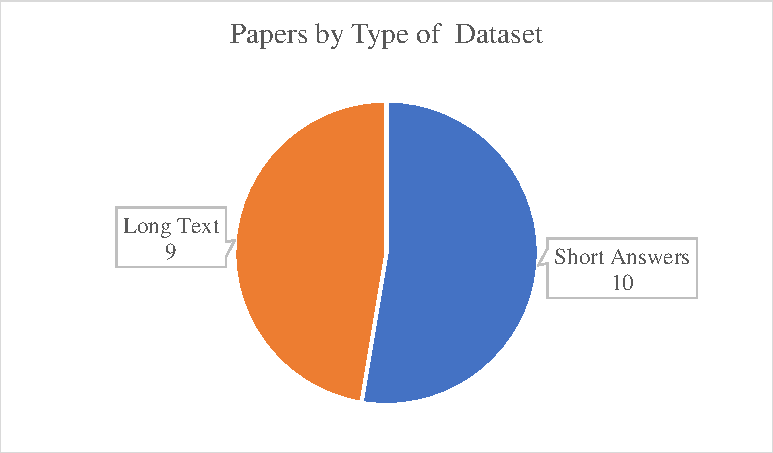
\includegraphics[width=0.5\linewidth]{img/papersbytype.pdf}
		\caption{Number of short Answer and number of long answer models}
		\label{shortlongcomparison}
	\end{figure}
	\subsubsection*{Short and Long Answer Approaches}
	Models designed for short answers often utilize different methodologies compared to those for long essay-style prompts. Short answers typically consist of a few structured sentences that address specific questions or facts, requiring less complex language processing. In contrast, essays are longer and more intricate, necessitating evaluation across multiple dimensions, such as content, coherence, grammar, and writing style. This complexity demands sophisticated models capable of capturing nuances in argumentation and organization.
	
	Most short answer models implement text similarity algorithms against a model answer, a technique that is not applicable to long essay texts. Long essay scoring systems must account for additional features, such as coherence and writing style. Some approaches are relevant to both short and long text systems, which will be categorized separately.
	
	\begin{figure}[H]
		\centering
		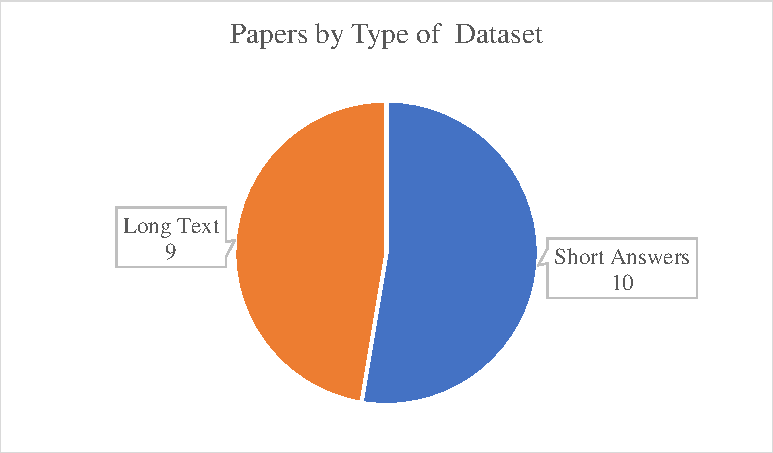
\includegraphics[width=0.5\linewidth]{img/papersbytype.pdf}
		\caption{Number of short answer and long answer models}
		\label{shortlongcomparison}
	\end{figure}
	
	\subsubsection*{Text-to-Text Similarity Algorithms}
	Text similarity algorithms compare students' responses with model answers or those from a training dataset. These algorithms include knowledge-based similarity, string-based similarity, corpus-based measures, and hybrid approaches, which aim to identify the degree of similarity between words based on extracted information. Hybrid methods combine various measures to generate a comprehensive similarity metric. Common approaches in literature focus on either lexical similarity (character similarity) or semantic similarity (meaning similarity).
	
	\begin{enumerate}
		\item \textbf{Knowledge-Based Similarity} \\
		Knowledge-based approaches use semantic networks to assess the similarity of ideas within the text. A commonly used database is WordNet, which has versions in various languages, including Arabic, Hindi, Bengali, and Persian.
		
		\item \textbf{Corpus-Based Similarity} \\
		This approach utilizes large corpora to measure semantic similarity between words. A prevalent technique is Latent Semantic Analysis (LSA), which posits that words with similar meanings occur in similar contexts. A term-document matrix, representing word counts per document, is created. Raw frequencies are transformed using weighting schemes such as TF-IDF:
		\begin{align*}
			\text{TF}(t, d) &= \frac{\text{Number of occurrences of term } t}{\text{Total number of occurrences in document } d} \\
			\text{IDF}(t, D) &= \log \left( \frac{\text{Total number of Documents in the Corpus } D}{\text{Total occurrences of the term } t} \right)
		\end{align*}
		The weight \( w \) is then determined by multiplying TF and IDF. LSA uses Singular Value Decomposition (SVD) to reduce the rank of the term-document matrix, allowing matrices for both documents to be compared via cosine similarity.
		
		However, LSA has limitations regarding contextual ambiguity; for example, the word "bank" can refer to a financial institution or the side of a river, leading to misrepresentation in latent space. Additionally, LSA treats text as a "bag of words," ignoring word order. Consequently, the phrases "The dog chased the cat" and "The cat chased the dog" would be treated similarly despite their opposite meanings. Furthermore, SVD's reliance on input data quality and quantity necessitates large, high-quality training datasets. Latent Semantic Indexing (LSI), an application of LSA, is primarily used for information retrieval.
		
		\textbf{DISCO} (Extracting Distributionally Similar Words using CO-occurrences) is a tool developed by \href{https://www.linguatools.de/disco/disco_en.html}{Linguatools}. It extracts distributionally similar words by analyzing co-occurrence data from a large text corpus, examining how frequently words appear together within a defined context window. DISCO constructs co-occurrence matrices and uses similarity measures such as cosine similarity or Jaccard similarity to quantify relationships between words. It ranks similar words based on co-occurrence patterns and similarity scores, supporting multiple languages, including Arabic, Czech, Dutch, English, French, German, Italian, Russian, and Spanish.
		
		\item \textbf{String-Based Similarity} \\
		This method evaluates the similarity of two strings based on their character composition and sequence. Some string-based similarity measures discussed include:
		\begin{enumerate}
			\item \textbf{Damerau-Levenshtein (DL) Distance} \\
			This measure calculates the minimum number of operations required to transform string \( S_1 \) into string \( S_2 \), where operations can include insertion, deletion, transposition of characters, or substitution of a single character. Normalization \cite{1_gomaa2014arabic} is performed to compute similarity.
			
			\item \textbf{Longest Common Substring (LCS)} \\
			This approach identifies the longest sequence of shared characters (substring) between two texts, which can be useful for detecting the presence of key ideas and references.
			
			\item \textbf{N-gram Similarity} \\
			An n-gram is a contiguous sequence of \( n \) items from a given text, which may include characters, words, or even phonemes. This sliding window approach can be applied at either the character or word level. The text is first split into smaller units (n-grams) of various sizes, allowing for counting matching n-grams or calculating Jaccard similarity:
			\begin{itemize}
				\item \textbf{Jaccard Similarity} \\
				$$J(A,B) = \frac{|A \cap B|}{|A \cup B|}$$
				where \( |A \cap B| \) is the number of n-grams common to both texts, and \( |A \cup B| \) is the total number of unique n-grams across both texts.
			\end{itemize}
		\end{enumerate}
	\end{enumerate}
	
	\textbf{Text Similarity and Dissimilarity Measures} \\
	Statistical methods are employed to identify the degree of similarity between two texts. Higher similarity indicates greater resemblance, while lower dissimilarity indicates closer alignment.
	\begin{itemize}
		\item \textbf{Cosine Similarity} \\
		For two vectors, cosine similarity provides the cosine of the angle between them:
		$$S_c(t_1, t_2) = \frac{t_1 \cdot t_2}{|t_1||t_2|}$$
		Here, the cosine similarity of text 1 and text 2 is the dot product of these vectors divided by the product of their magnitudes. The value ranges from 0 (least resemblance) to 1 (most resemblance).
	\end{itemize}
	
	\subsection{Model Evaluation Metrics} 
	
	\subsubsection*{Kappa Score}
	The Kappa Score, also known as Cohen's Kappa Statistic, measures the agreement of classification models. It is more reliable than simple agreement measures because it accounts for the possibility of chance agreement. The observed agreement \( P_o \) represents the proportion of similar scores assigned by human raters and the AES system, while \( P_e \) denotes the hypothetical chance of agreement based on the probability of both raters randomly assigning the same score. The Kappa Score is calculated as follows:
	$$ k = \frac{P_o - P_e}{1 - P_e} $$
	
	\subsubsection*{Quadratic Weighted Kappa}
	Quadratic Weighted Kappa improves upon the traditional Kappa by considering not only the presence of agreement but also the severity of disagreement between raters. While Kappa applies to nominal variables, Quadratic Weighted Kappa is suitable for ordinal variables, where categories have a defined order. After calculating \( P_o \) and \( P_e \), these values are multiplied by a weights matrix to reflect the seriousness of disagreement between human and AES ratings. Weights can be defined linearly or quadratically. 
	
	The weight \( W_{i,j} \) is determined using the following formulas:
	\begin{align*}
		W_{i,j} &= 1 - \frac{|i - j|}{n - 1} \\
		W_{i,j} &= 1 - \left( \frac{i - j}{n - 1} \right) ^2
	\end{align*}
	Here, \( n \) represents the number of possible categories or ratings. The weight calculation is influenced by \( |i - j| \), where \( i,j \in \{ 1, 2, 3, \ldots, n \} \). A greater score difference results in a smaller weight. Most evaluations utilize the Quadratic Weighted Kappa (QWK).
	
	Using the weight matrix \( W \), observed frequency matrix \( O \), and expected frequency matrix \( E \), the score is computed as follows:
	$$ k_W = \frac{\sum_{i,j} W_{i,j} \cdot O_{i,j} - \sum_{i,j} W_{i,j} \cdot E_{i,j}}{1 - \sum_{i,j} W_{i,j} \cdot E_{i,j}} $$
	
	\subsubsection*{Precision}
	Precision is defined as the proportion of correctly identified positive results among all results predicted to be positive. In AES, precision measures the accuracy of the system's decision to assign a particular score (e.g., a high grade or a pass):
	$$ \text{Precision} = \frac{TP}{TP + FP} $$
	
	Where:
	- \( TP \) is the number of true positives (correctly predicted positives),
	- \( FP \) is the number of false positives (incorrectly predicted positives).
	
	\subsubsection*{Recall}
	Recall, also known as sensitivity, refers to the ability of a model to identify all relevant cases (positives). In AES, recall assesses the model's ability to accurately score work that should have received a specific grade:
	$$ \text{Recall} = \frac{TP}{TP + FN} $$
	
	Where:
	- \( FN \) is the number of false negatives (missed positives).
	
	\subsubsection*{F1-Score}
	The F1-Score is the harmonic mean of precision and recall. It provides a balance between these two metrics, useful when class distribution is uneven:
	$$ F1 = 2 \cdot \frac{\text{Precision} \cdot \text{Recall}}{\text{Precision} + \text{Recall}} $$
	
	This metric is particularly relevant in AES contexts where both precision and recall are critical for assessing the quality of scoring systems.
	
	\subsection{Short Answer Scoring}
	
	%\subsubsection*{Hybrid Approaches}
	\textbf{\textcite{1_gomaa2014arabic}} (Arabic) combines string based, corpus based, and knowledge based similarity measures. String similarity is calculated using LCS (Longest Common Subsequence). They performed normalization tasks as well. They also calculated DL distance. They used character-based and word-based N-gram similarity was calculated and determined that character-based N-gram performed better in their model overall. 
	For corpus based measure, the paper utilizes DISCO. For measuring knowledge based similarity, the paper translated the dataset into English and the semantic similarity was measured through the English WordNet instead of the Arabic version, because of weak word coverage in the Arabic WordNet. They claimed translation helped improve the results of the model. An improved version of the Arabic WordNet, however, has been released since then. \\ They also introduced a sentence level semantic similarity measure. The system computed sentence-level semantic similarity using the Bag of Words model and they created a similarity matrix of word pairs between student and model answers. A matrix captured individual word similarities to calculate an overall score. \\ The paper showed a correlation between examiners of 0.86 and correlation between the model and examiner was 0.83. They also compared different translators and results showed human translation to be better than Bing or Google when applying string based similarity measures on translated text. Performance of Google and Bing translation was close to each other. They proposed a CombineBest method to determine the features that provided the best correlation and then used SMOReg (A variant of Support Vector Machine algorithm similar to \textcite{4_abdeljaber2021wordnet}) and Linear regression to obtain best Pearson correlation of 0.83. Best RMSE value of 0.75 was obtained by applying SMOReg on CombineBest method. In comparison, the Pearson correlation and RMSE between two annotators was 0.86 and 0.69 respectively. \\
	
	\textbf{\textcite{2_shalabi2016levenshtein}} (Arabic) uses a similar approach by first carrying out heavy stemming and then determining the weight of each word by calculating the Levenshtein (DL) distance. After determining the weights of the words in student answer, the model looks for presence of that word in the final answer. If there is some level of similarity, the weight of that word is added to the final score. The paper only dealt with string-based similarity measure. \\
	
	\textbf{\textcite{3_shehab2018arabicsimiliarity}} (Arabic) proposed a Bag of Words Model to determine the final score. The paper experiments with using Levenshtein (DL) distance and N-gram for  string similarity and LSA and DISCO for corpus based similarity measure. Their experimental results showed that N-gram based measures gave the highest correlation (0.820) out of the 4 similarity measures. DL was 2nd (0.800), and the corpus based measures DISCO and LSA were third (0.796) and fourth (0.796) respectively. \\
	
	\textbf{\textcite{8_abdel2021lcs}} (Arabic) uses LCS (longest common subsequence) 
	Arabic WordNet provides synonyms, which improves the accuracy of the model. The paper uses a modified approach of LCS using a weight based measurement technique.
	It also discusses the limits of Arabic WordNet due to limited coverage, so certain plural forms don't work in AWN. To deal with this issue, stem of model answer and stem of synonyms used to determine whether they lie in the common ``synset"
	
	The problem of standard LCS is that certain student answers can give a similar score with some model answers that are much closer to model answers syntactically. For this, the model not only uses contiguity of LCS for certain substrings in model answer and student answer, but also considers contiguity of all common subsequence of these texts. This turns the LCS to LCCS (longest common contiguous sequence) - The value for LCCS is also normalized. The final results obtained were $r$ of 0.94 and RMSE of 0.81. According to them, they were able to outperform other LCS models by utilizing Arabic WordNet as well as using LCCS instead of LCS. \\
	
	\textbf{\textcite{16_rababah2017short}} (Arabic) also applies LSA against a model answer. During their preprocessing, they aimed to improve the accuracy by presenting a hybrid method to verify the correctness of extracted stems by using multiple stemmers and WordNet. Their model consisted of making a term document matrix, applying TF-IDF to determine word weights, and measurement of score using cosine similarity. They achieved a 95.4\% percent correlation. They used a recall based approach (precision, accuracy, f-score) and found 62\% correlation when using R-call based scoring. \\
	
	\textbf{\textcite{27_gaheen2021jaya}} (Arabic) proposed a neural based approach. After preprocessing, a word by context (WCM) matrix is built to perform LSA. Then, they created a multi-layer perceptron network (MLP). Elitist-Jaya optimization algorithm was used to optimize the network. This process involved generating random vectors that are evaluated to optimize the neural network. They also experimented with various other optimization algorithms. The model achieved an average 0.987 correlation using eJaya, followed by DE (Differential evolution), MVO (Mean-Variance Optimization), and PSO (Particle Swarm Optimization). eJaya outperformed a conventional neural network by 7\% . 
	\subsubsection*{Feature Extraction using Support Vector Machine}
	Support Vector Machines (SVM) work by mapping data into a high-dimensional space, where each feature corresponds to an axis. A linear classifier is then trained by finding a hyperplane that separates positive and negative instances. The direction of this hyperplane is determined by the support vectors—key data points that define the decision boundary.
	
	Feature selection in SVM aims to retain only the most important features that contribute to accurate classification. One common method is the F-score, which evaluates how well each feature differentiates between two classes (positive and negative). Features with higher F-scores are considered more significant. Other methods, like Recursive Feature Elimination (RFE) or mutual information, can also be used to rank and select features based on their contribution to the model's performance. \\ 
	
	\textbf{\textcite{4_abdeljaber2021wordnet}} (Arabic) used SVM with F-score measure to select the important features to score short answers. In addition, it used the Arabic WordNet to determine synonyms. Finally, the score is generated using cosine similarity of model answer and student answer matrices. They achieved $r$ of 0.99 with Arabic WordNet and 0.98 without the WordNet.
	
	\subsubsection*{Transformer Approach in Short Answer Scoring}
	\textbf{\textcite{22_meccawy2023mining}} (Arabic) also experimented with different approaches. They used ARASAG and \textcite{16_rababah2017short}'s dataset. FARASA was used for light stemmming and ISRI stemmer was used for base stemming. One approach was to use the Arabic WordNet to consider synonyms and then semantic similarity by cosine similarity. The second approach was to utilize Word2Vec. It is a word embedding technique that presents words as vectors in a vector space and the closer the words are, the greater the similarity of their meanings. AraVec was used as the Word2Vec model. The third approach as to use BERT based approach, utilizing AraBERT. Cosine similarity was used for the similarity measure. Their methods performed better overall when using light stemming. The best RMSE achieved was through BERT (1.04), which was significantly better than any other method. Best $r$ was obtained by using Word2Vec (0.78) in ARASAG dataset. The same model, when trained and applied on the Rababah's dataset, achieved greater $r$ (0.84) and performed slightly better with base stemming approach. \\
	
	
	\textbf{\textcite{23_ghazawi2024bert}} (Arabic) has introduced AR-RES, one of the largest publicly available datasets for Arabic AES. The dataset consists of questions and answers from different topics, divided by genders as well. They utilized ISRI stemmer for their preprocessing and the AraBERT tokenizer for tokens. After training the model on AraBERT their model achieved a QWK score of 0.884 and an F1 score of 0.78. The performance of their model exceeded in some topics than others. They explained this to be because of the complexity of certain topics: the model showed lower performance in topics like Management Information Systems, where the course had more open-ended answers while answers in courses like Chemistry were source dependent and controller and therefore the model performed better. 
	
	\subsection{Long Text Essay Scoring}
	\subsubsection*{Measure of Coherence with Discourse Analysis}
	Two common methods to determine coherency of an essay are Rhetorical Structure Theory (RST) and Segmented Discourse Representation Theory (SDRT). \\ In RST, texts are divided into segments called "nuclei" (central ideas) and "satellites" (supporting ideas), which are connected through rhetorical relations, such as cause-effect, contrast, or elaboration. These relations describe how different sections of a text interact to form a cohesive argument or narrative. 
	
	\textbf{\textcite{6_ghamdi2014hybridarabic}} (Arabic) presented Abbir, a hybrid AEE for essays in Arabic language. They built an LSA concept space and also measured surface level features by measuring spelling mistakes and number of words. In the training phase, the LSA concept space was built using a training dataset and the LSA distance. Best result achieved by including LSA with stemming, word distance, and spelling mistake distance was $r$ of 0.78 and RMSE of 0.89. Their threshold value $t$ was set to be 17\% of the overall score. 
	
	\subsubsection*{Rule based approaches}
	\textbf{\textcite{7_qahtani2019rulebased}} (Arabic) used MADAMIRA \cite{pasha2014madamira} for morphological analysis during preprocessing for part-of-speech tagging and stemming words. Spelling errors were identified using FARASA spell checker. The paper also considers structure of essay by considering the essay to be divided into introduction, main body, and conclusion. Coherence of the answers was measured by counting discourse connectives. They also measured checked for punctuation marks and style level by counting frequency of repeated words. Threshold was set for 16\% of the overall score. 73\% of the scores were considered to be within acceptable range.
	
	
	\subsubsection*{Transformer Model and Deep Learning approaches}
	Text classification is difficult in many such languages because of the lack of available scored datasets. This is where, the deep learning method can help address such problems. One of the significant advantages of using transformer architecture over deep learning models is that they are less susceptible to vanishing gradient problem. They rely on attention mechanism rather than sequential processing used in RNNs or LSTMs. They are able to capture relations of text input in context to other text inputs. \\
	
	
	\textit{BERT} \\
	Bidirectional Encoder Representations from Transformers is an open-source machine learning framework utilized in many NLP applications. It uses a transformer based neural network to generate human-like language. A conventional transformer model consists of encode and decoder modules but BERT has an encoder-only architecture, meaning it works mainly in understanding the input sequences rather than generating the output. \\ BERT is pretrained on large amount of unlabelled data, where it learns contextual embeddings. It can be fine by training on labelled data. \\ While traditional models work by processing text in one direction, BERT works by using a bidirectional approach: The model analyzes the text from both directions. This way, it is able to generate embeddings that are deeply contextualized. Improved model understanding allows for better assessment of coherence, relevance and precision of arguments in an essay. Since such architecture can capture more comprehensive context, it can be better at generalizing different writing styles and improve reliability of the scoring in comparison to unidirectional encoder. It uses MLM (masked language model) and next sentence prediction when training in order to easily define a prediction goal. RoBERTa also uses self-attention to evaluate input sequences and construct phrase-level contextual representations. It is arguably more effective because it is primarily trained on a larger dataset (160gb) in comparison to BERT (16GB) \\
	
	\textbf{\textcite{9_firoozi2024bert}} (Persian) uses multilingual BERT (mBERT) to score long essays. First they built a model using a Word Embedding Model using Word2Vec. In Word2Vec, words are represented as vectors of real numbers, where semantically similar words have similar vector representations. This model was used for comparison against mBERT model. After fine tuning the mBERT, they were able to achieve kappa score, QWK and accuracy of 0.93, 0.84, and 73\% respectively. This was significantly better than the word embedding model where they achieved Kappa score, QWK and accuracy of 0.82, 0.75 and 71\% respectively. Their model performed well with various levels of text difficulty but the performance dropped in grading advanced level essays. \\
	
	
	\textit{Deep learning and LSTM} \\
	Long short term memory, usually employed in preprocessing stage, used for semantic analysis. This architecture helps model to recognize the temporal dependencies and patterns within the text data. LSTM can provide unique strengths when dealing with long texts consisting of sequential data. It is a type of recurrent neural network (RNN) that aims to solve the vanishing gradient problem in neural networks. Hence it plays a key role in capturing long-range dependencies in the data. LSTMs have a memory cell that can store and retrieve information over long periods of time. Hence not only storing relationships between words and certain phrases but also flow of ideas in a response. \\
	
	\textbf{\textcite{10_singh2023hindi}} (Hindi) thoroughly documented the various approaches for their model. They experimented with Linear Regression, Support Vector Regression (SVR), RandomForest and XGBoost for classification and regression approach. They extracted features like essay length, average word length, readability, vocabulary, and semantic overlap and coherence. They calculated readability scores using \cite{sinha2012new} and vocabulary score by counting out-of-vocabulary words. mBERT is used to measure semantic similarity of two sentences at a distance of four sentences. \\ For building a neural-network based architecture,  they experimented with a total of 4 neural-based approaches. \\ The BiLSTM method consists of two LSTMs processing the sequence in both forward and backwards direction. CNN (Convolutional Neural Network) was used to capture short dependencies over a fixed window size. The also combined CNN to extract features from the text and then used LSTM for to process sequences. They attached an attention layer to it. Their fourth neural approach was to implement SKIPFLOW Model \cite{tay2018skipflow}. This novel approach calculates coherence by reading LSTM networks. \\ They also fine tuned a number of transformer models: Multilingual BERT (mBERT), DistilmBERT, XLM-Roberta, MuRIL, and IndicBERT. Their dataset consisted of both an organic corpus and a translated corpus from the ASAP dataset. Overall, their methods were able to show more consistent results with translated texts. From regression appraoches, XGBoost provided the best results with QWK score of 0.827 in organic corpus. Different regression approaches had a large variation in their QWK scores (0.579 - 0.827) when working in organic corpus. Neural based approaches, however, had a higher average with BiLSTM providing the best results (0.842) followed by CNN + LSTM + Transformer (0.827) and SKIPFLOW (0.812). Transformer based models were able to provide the best results with mBERT scoring 0.852: highest for evaluating organic corpus. \\
	
	\textbf{\textcite{11_walia2024hybrid}} (Hindi) used a similar approach to \textcite{10_singh2023hindi}, utilizing LSTM and a transformer model. They implemented a Hybrid PSO (Particle Swarm Optimization) based approach for LSTM and RoBERTa. The model achieved an overall accuracy of 95\%. Details of the datasets, however, were not shared.
	
	\subsubsection*{Information Retrieval Approaches}
	\textbf{\textcite{17_abbas2015svm}} (Arabic) focuses on VSM and Latent Semantic Indexing in web-based learning. Information retrieval (IR) is applied to extract information from the text. Each query for IR  The idea behind VSM is to represent each essay as a vector as a point in space. \\ Similarity between the vector and the query is done through matching functions. The model generates an vector for each essay and for each query from sets of terms with their weights. The weight of each term is identified through TF-IDF. Then, the cosine similarity between the vector for the query and the vector of the essay is measured. \\ In the second stage of the model, they implemented LSI, where they built the term document matrix. Instead of performing SVD, they performed truncated SVD, which they claimed, could help reduce noise and remove unnecessary information for their application. The result for the LSI score is found by cosine similarity between the LSI vector (after truncated SVD) and a query (vector consisted of terms for the query). As new documents get added to the LSI space, the term document matrix needs to be recalculated. Instead of rebuilding the matrix from scratch, they suggested folding in to reconstruct the matrix. The final score generated was the average of the VSM score and the LSI score. The dataset used in the study was not large, consisting of 30 essays. Their model correctly scored 23/30 essays. They achieved a correlation of 0.978. \\
	
	
	\textbf{\textcite{24_islam2013abess}} (Bengali) also built a model utilizing information retrieval and GLSA (generalized latent semantic analysis). They created an n-gram document matrix by first determining the index terms. The n-grams are weighted by multiplication of frequency of n-grams by n. Then, SVD is carried out on the n-gram document matrix. A query matrix is created from a submitted essay and cosine similarity of the query vector with with term-document matrix determines the grade. They achieved precision and recall of 98\%. 
	
	\subsubsection*{Hybrid Approaches in long essay systems}
	\textbf{\textcite{5_aljouie2017schoolchildren}} (Arabic) uses LSA of the student answer against the training dataset. It uses RST to determine 40\% of the score, LSA for 50\% of the score, and 10\% of the score is measured by spelling mistakes. \\ They set the threshold to be 1.5 marks and achieved an accuracy of 78.33\% \\
	
	
	\textbf{\textcite{18_alqahtani2020svr}} (Arabic) categorized the features extracted from the text into surface level (quantitative measures for counting words), syntactic (presence of POS and mistakes), lexical (presence of certain keywords, punctuation features etc.), semantic (using Arabic WordNet and word embedding) and discourse (identifying discourse connectives). In the first part of the paper they presented a thorough list of features that they were able to extract from the text. In the second part of their paper, they proposed 4 models.
	\begin{enumerate}
		\item Spelling model. Necessary features were identified and the FARASA spell checker was used. They also assessed the performance of FARASA on their dataset where there was cases where it failed to correct the mistake (3.4\%) or corrected a word that was already correct (10.1\%). At $t = 17\%$ and $t = 25\%$, it achieved $r$ of 0.65, 0.72 respectively.
		\item Structure model identified structure of the text using surface level and some lexical features like presence of keywords. At $t = 17\%$ and $t = 25\%$, it achieved $r$ of 0.74, 0.86 respectively.
		\item Coherence model used discourse features and surface level features to identify how well the sentences are linked together. At $t = 17\%$ and $t = 25\%$, it achieved $r$ of 0.65, 0.69 respectively.
		\item Style model uses morphological and surface level features to find word repetition, number of synonyms, number of discourse connectives. At $t = 17\%$ and $t = 25\%$, it achieved $r$ of 0.57, 0.65 respectively.
		\item Punctuation marks model used punctuation and discourse features to determine correct usage of marks. At $t = 17\%$ and $t = 25\%$, it achieved accuracy of 90\% and 96\% respectively. 
	\end{enumerate}
	Overall, the model achieved 96\% accuracy and 0.87 correlation. \\
	\textbf{\textcite{26_alsanie2022threelevels}} (Arabic) worked by improving the existing model by \textcite{6_ghamdi2014hybridarabic}. The model evaluated the essay’s style in terms of syntactic structure and spelling, while analyzing its content through lexical semantics. A context-free grammar model was employed; however, due to the need for language contextualization and the difficulty in distinguishing between salient and anomalous language constructs, the model was lexicalized and enhanced with probabilistic rule choices, converting it into a stochastic lexicalized context-free grammar. Sub-tree kernels and Support Vector Machines (SVMs) were used for syntactic measurements, with flexibility in the SVM to account for dataset uncertainty. Latent Semantic Analysis (LSA) was also applied, and logistic regression was used to determine the final score. The model outperformed \textcite{6_ghamdi2014hybridarabic} and achieved best QWK of 0.68 and accuracy of 51\% while \textcite{6_ghamdi2014hybridarabic}'s model achieved best QWK and accuracy of 0.34 and 44\%, respectively.

	
	\section{Discussion}
	
	\begin{center}
		\begin{tikzpicture}[
			level 1/.style={sibling distance=28em, level distance=5em},
			edge from parent/.style={draw, -latex, edge from parent path={
					(\tikzparentnode.south) -- ++(0,-1.2em) -| (\tikzchildnode.north)}},
			every node/.style = {shape=rectangle, rounded corners,
				draw, align=center, fill=white, inner sep=1em}
			]
			
			% Root node (top of the hierarchy)
			\node {AES Methods}
			child { node {Short Answer (10)} }  % First child
			child { node {Long Text (9)} };     % Second child
			
		\end{tikzpicture}
	\end{center}
	
	\begin{table}[H]
		\begin{tabularx}{7in}{|X|m{0.8in}|m{0.8in}|}
			\hline
			\multirow{2}{*}{Common Approaches} & \multicolumn{2}{c|}{Number of papers} \\ \cline{2-3}
			& Short Answer & Long Text \\ \hline
			String Based Similarity (Including N-gram, LCS, DL Distance) & 8 & 1 \\
			Corpus Based Similarity (Including LSA, LSI, DISCO) & 6 & 3 \\
			Knowledge Based Similarity (Utilizing WordNet for Synonyms) & 4 & 1 \\
			Support Vector Machines (Including classification and regression) & 2 & 3 \\
			Transformer Models & 2 & 3 \\
			Neural Based Approaches & 1 & 2 \\ 
			\hline
		\end{tabularx}
		\caption{Number of Papers Utilizing Each Method}
		\label{tab::papertypes}
	\end{table}
	Table \ref{tab::papertypes} presents the number of papers that assessed and employed specific techniques in their research, considering those that utilized multiple approaches. While string-based methods were computationally efficient, they failed to capture semantic meaning. Consequently, the majority of papers employed this approach in conjunction with a semantic measure. \\
	
	Many studies utilized Latent Semantic Analysis (LSA) as a primary method for measuring corpus-based similarity. LSA constructs a term-document matrix representing the frequency of terms across a set of documents. However, LSA and its extension, Latent Semantic Indexing (LSI), typically require reprocessing the entire matrix and recalculating the singular value decomposition (SVD) matrix. When dealing with large matrices, this operation can be computationally expensive, posing significant challenges for large-scale datasets. In contrast, scalable approaches using deep learning and transformer models, such as BERT and GPT, may effectively address this problem by handling semantic relationships without relying on explicit matrix factorization. \\
	
	\textcite{17_abbas2015svm} proposed a workaround to LSA’s computational limitations by employing a "folding-in" method. Instead of recalculating the entire SVD from scratch whenever a new essay is added, the new essay is projected onto the existing LSA space using the original SVD components. This significantly reduces computational overhead. \\
	
	However, LSA’s bag-of-words nature introduces another limitation: it cannot capture word order or syntactic nuances. This inability to differentiate between sentences containing the same words in a different order can impact the model's accuracy, especially when student answers use similar words as model answers but convey entirely different meanings. For instance, "The essay argues against X" versus "The essay argues for X" would be treated similarly by an LSA-based system, despite conveying opposite meanings. \\
	
	To address some of these issues, \textcite{26_alsanie2022threelevels} combined LSA with a parser algorithm to analyze sentence structure and dependencies, enabling a more refined assessment of the essay’s content. \\
	
	Recent advancements in AES have shifted towards the use of deep learning models, particularly those based on neural networks and transformers, which better account for word order, context, and semantic relationships. \\
	
	Support Vector Machines (SVM) have been utilized for both classification and regression tasks in AES, particularly in systems involving scoring rubrics. SVMs are well-suited for tasks where the feature space is relatively well-defined, such as specific grading categories (e.g., grammar, coherence). However, the performance of SVMs can degrade when the feature space is large or noisy, which is often the case in long-text essays containing diverse expressions and stylistic variations. To address these challenges, some studies have proposed less rigid implementations of SVM \cite{17_abbas2015svm}, allowing for greater flexibility in the presence of dataset uncertainty. \\
	
	Transformer models, such as BERT and its variants, which are pre-trained on large text corpora, offer scalability by processing text in a parallelized manner and fine-tuning on essay-specific tasks. Multilingual models can be applied across various applications, making the technique more transferable than others. However, training these models is resource-intensive and requires a substantial corpus. Current assessments of BERT's performance by \textcite{9_firoozi2024bert} indicated a decline in effectiveness when evaluating advanced-level essays. 
	
	\section{Conclusion}
	
	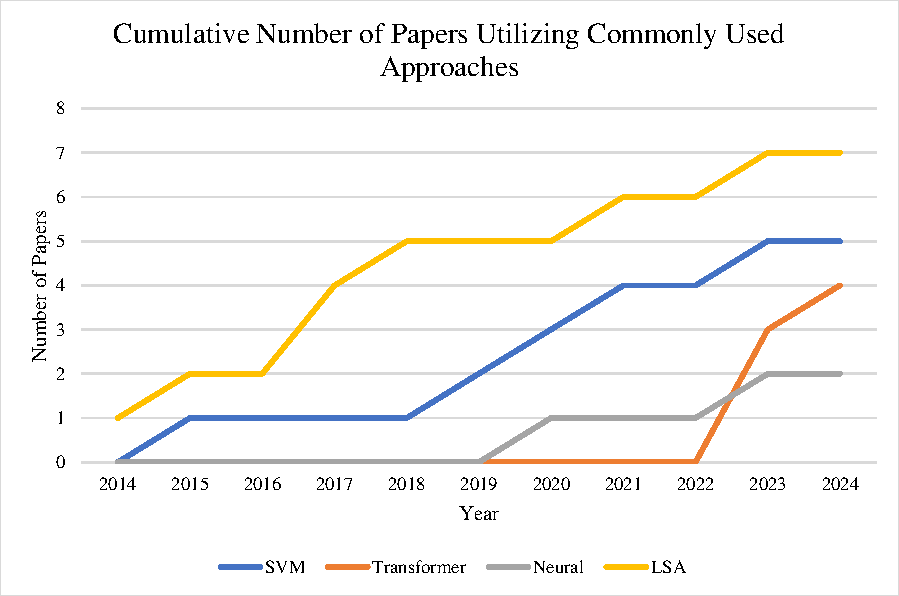
\includegraphics{img/paperstrend.pdf}
	
	In conclusion, the future of AES for low-resource languages appears promising, although challenges remain. The primary challenge is the limited availability of training datasets. The graph illustrates that traditional techniques, such as corpus-based similarity methods like LSA, have dominated over time. However, the emergence of transformer architectures has led to a notable increase in deep learning and transformer-based approaches due to their superior capacity for semantic measurement. We anticipate that ongoing advancements will make these powerful models more accessible and effective for low-resource languages, ultimately improving the accuracy and fairness of AES systems across diverse linguistic contexts. \\
	
	Coupling scores with feedback is essential for enhancing the learning experience. Providing detailed explanations for scores is crucial, as it significantly benefits learners. A significant drawback observed in the literature is the lack of feedback and explanations accompanying grades. Many studies relied on translating datasets instead of utilizing organic corpora, potentially affecting result quality. The general scarcity of datasets exacerbates these issues. Addressing these concerns by integrating comprehensive feedback and improving dataset availability will be critical for developing more effective and equitable AES systems.
	
	
	% \bibliographystyle{IEEEtran}
	\printbibliography
	% \bibliography{ref.bib}
\end{document}
